% Start of Chapter 1 - System Analysis
An inverted pendulum can be represented as a rigid body pendulum connected to a cart moving on a horizontal axis. Controlling the stability of the Zumobot can be compared to balancing the inverted pendulum on the moving cart.

\begin{comment}	% Commented out, for future usage of the code
	\begin{figure}[!htbp]
		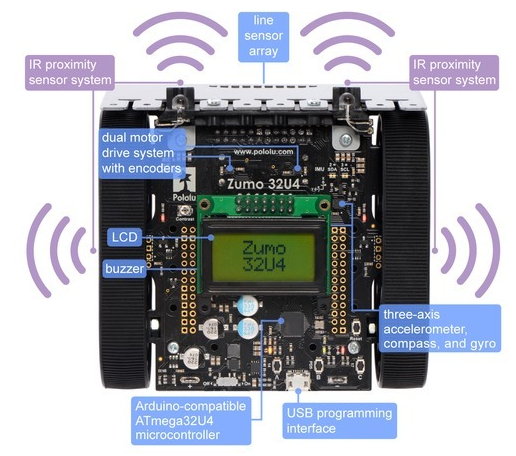
\includegraphics{img/zumo-superior.png}
		\centering
		\caption{Superior view of the zumo robot.}
		\label{fig:sup-zumo}
	\end{figure}
\end{comment}

%The figure \ref{fig:sup-zumo} shows the robot that will be modeled as a Wheeled Inverted Pendulum.

\begin{comment}	% Commented out for future usage of the code
	\begin{table}[!htbp]
		\centering
		\caption{Basic table.}
		\label{tab:tab1}
		\begin{tabular}{ccc}

			\toprule

			header A & header B & header C\\

			\midrule

			a & b & c\\
			c & d & e\\
			f & g & h\\

			\bottomrule

		\end{tabular}
	\end{table}
\end{comment}

%Text of the section\footnote{\label{fn1}This is a footnote}.

%Text of the section after the footnote \ref{fn1}.

TODO: Complete.
